\subsubsection{Evaluation For the HAC Agents}

The evaluation strategy is designed to assess the performance of the Human-AI Collaboration (HAC) system in terms of control stability and trajectory tracking capability. Two representative control tasks were defined: a vertical hovering task and a synthetic path following task. These tasks were selected as simplified proxies to evaluate the underlying control effectiveness without requiring full mission complexity.

\paragraph{Hovering Task}

The hovering task evaluates the system's ability to maintain stable altitude control. The objective is to regulate the drone's vertical position ($y$) within a predefined tolerance band $[H - R, H + R]$, where $H$ represents the target altitude and $R$ defines the acceptable deviation range.

Performance is monitored through both positional stability and qualitative visual feedback. A color-coded indicator system is used to provide real-time feedback on control states: yellow indicates the drone is below the target range, orange indicates it is above the range, and blue indicates stable hovering within the acceptable band (see \cref{fig:train}). This visualization supports rapid assessment of control stability during operation.

\begin{figure}[H]
    \caption{Real-time feedback visualization during hovering evaluation.}\label{fig:train}
    \centering
    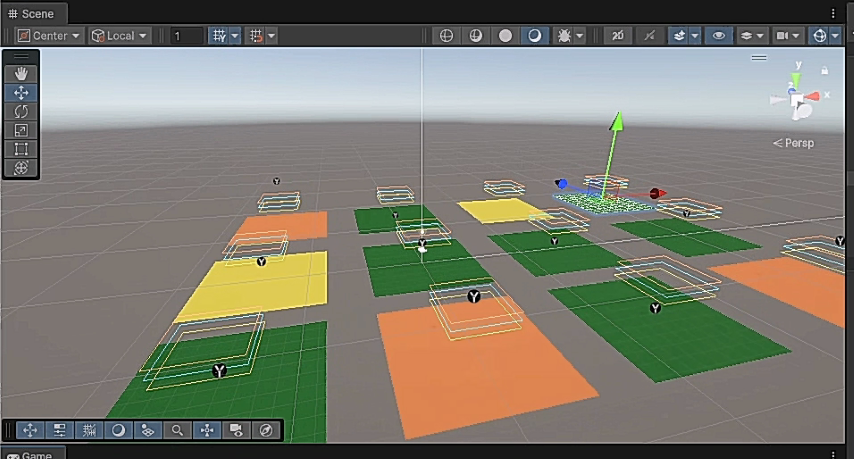
\includegraphics[width=0.8\linewidth]{img/train.png}
\end{figure}

The primary evaluation criterion for this task is the duration and consistency of maintaining the drone within the acceptable altitude band, which reflects the stability of the control system.

\paragraph{Path Following Task}

The path following task is introduced as a controlled synthetic trajectory tracking problem to evaluate the system's ability to follow predefined spatial references. This task is not intended to represent a realistic mission scenario, but rather to test the responsiveness and coordination of the control system under structured motion constraints.

A smooth trajectory is generated using cubic Bézier curves defined by four control points $P_0, P_1, P_2, P_3$, forming a round-trip path from the home position to a target waypoint and back. The trajectory is defined as:

\begin{equation}\label{eq:bezier}
    B(t) = {(1-t)}^3 P_0 + 3{(1-t)}^2 t P_1 + 3(1-t) t^2 P_2 + t^3 P_3, \quad t \in [0,1]
\end{equation}

The resulting path provides a continuous reference trajectory for evaluating tracking behavior. The geometric structure of the generated path is shown in \cref{fig:path_design}, where asymmetric control point offsets are used to create directional variation between outbound and return segments.

\begin{figure}[H]
    \caption{Synthetic path structure used for trajectory tracking evaluation.}\label{fig:path_design}
    \centering
    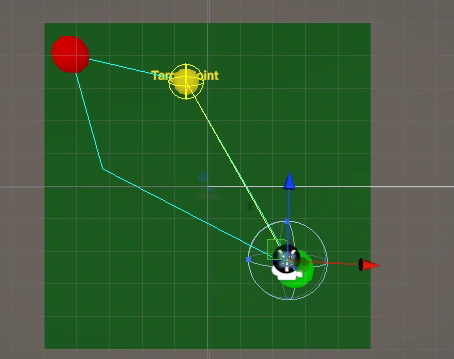
\includegraphics[width=0.8\linewidth]{img/path.png}
\end{figure}

Evaluation in this task focuses on trajectory tracking performance, including deviation from the reference path and stability of directional control during transitions between waypoints. 

\paragraph{Evaluation Environment}

To ensure consistent comparison across tasks, both hovering and path following evaluations are conducted in a non-XR visualization environment. System behavior is projected onto a flat-panel interface, allowing direct observation of control signals and system responses without requiring immersive hardware. This setup ensures reproducibility and simplifies performance analysis across experimental runs.